\subsubsection{Model performance}
\label{sub:comb_performance}

\outline{Section will only cover DM2 results, summary of result evolution
will be given in following section}

\begin{table}
  \begin{tabular}{lrrrrrrr}
    \toprule
    & \multicolumn{4}{l}{Classification} & \multicolumn{3}{l}{Regression} \\
    \midrule
    Data set & CCE & Acc & Ret Acc & Fav Acc & MAE & Ret MAE & Fav MAE \\
    \midrule
    Celebrities & 0.80 & 65.16\% & 61.91\% & 68.40\% & 3,286.16 & 1,438.98 & 5,133.35 \\
    Politicians & 0.82 & 65.34\% & 64.22\% & 66.46\% & 447.61 & 262.78 & 632.44 \\
    Companies & 0.62 & 73.52\% & 75.88\% & 71.15\% & 19.41 & 10.99 & 27.84 \\
    Combined & 0.76 & 68.42\% & 70.05\% & 66.79\% & 401.52 & 201.70 & 601.33 \\
    \bottomrule
  \end{tabular}
  \caption{Summary of results for multi-input deep neural networks}
  \label{tab:deep2_results}
\end{table}

\structure{Description of overall results}
\outline{Classification perf on similar level for all data sets (loss values
between 0.62 and 0.82)}
\outline{Overall classification accuracies between 65 and 75 percent}
\outline{Best performance on company data set (which is most imbalanced)}
\outline{Notable differences between RetAcc and FavAcc, biggest difference for
celebrities (6.49\%), smallest for politicians (2.24\%)}
\outline{On first glance, classification performance is not dependent on data set size}
\outline{Validation metrics are listed for best generalizable model}
\outline{Ignoring overfitting, accuracies of more than 90\% are achievable on
all data sets}
\outline{Regression results on different magnitudes (as expected)}
\outline{Retweet predictions are more generally more accurate than favorite
predictions (notable difference, about three times bigger for all data sets)}

\begin{figure}[h]
\begin{subfigure}{.5\textwidth}
  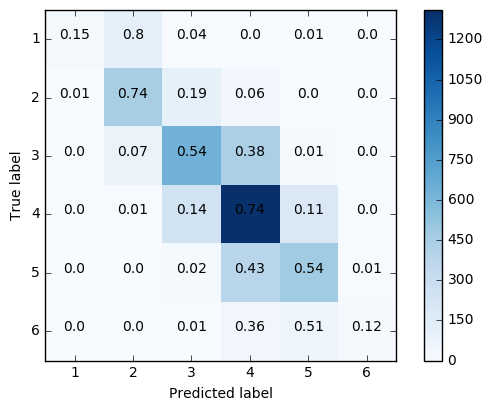
\includegraphics[width=.95\linewidth]{img/celeb_d2_cm_retweets}
  \caption{Celebrity data set}
  \label{fig:retw_distr_sub1}
\end{subfigure}%
\begin{subfigure}{.5\textwidth}
  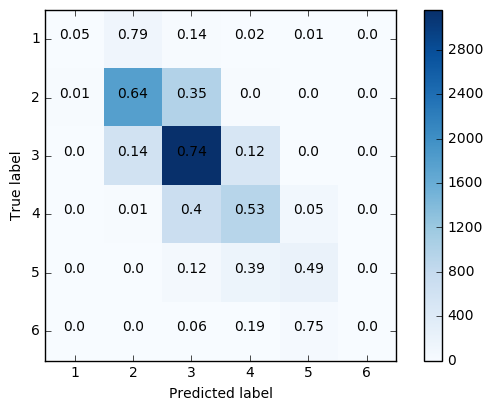
\includegraphics[width=.95\linewidth]{img/polit_d2_cm_retweets}
  \caption{Politician data set}
  \label{fig:retw_distr_sub2}
\end{subfigure}
\begin{subfigure}{.5\textwidth}
  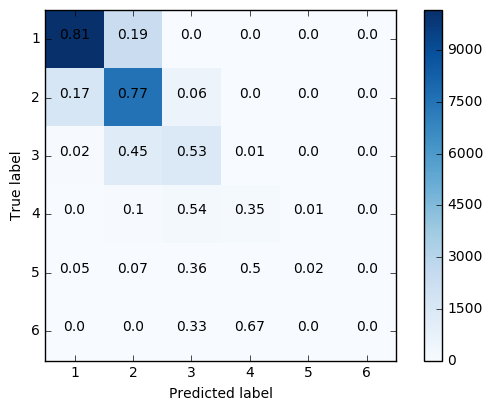
\includegraphics[width=.95\linewidth]{img/corp_d2_cm_retweets}
  \caption{Company data set}
  \label{fig:retw_distr_sub3}
\end{subfigure}%
\begin{subfigure}{.5\textwidth}
  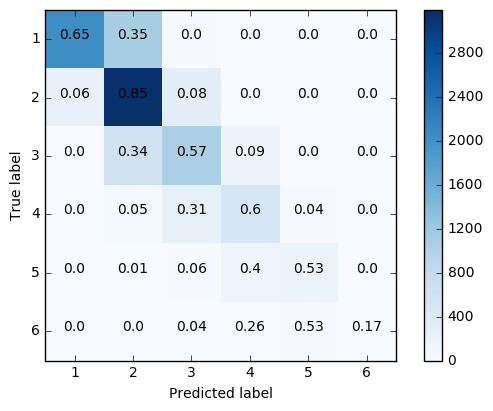
\includegraphics[width=.95\linewidth]{img/comb_d2_cm_retweets}
  \caption{Combined data set}
  \label{fig:retw_distr_sub4}
\end{subfigure}%
\caption{Confusion matrices for multi-input deep neural networks}
\label{fig:d2_cm}
\end{figure}

\structure{Description of classification results}
\outline{Specialized data sets: class accuracies above 50\% for three of four
classes}
\outline{Best performance on company data set mainly stems from strong performance
on most popular classes (acc around 80\%)}
\outline{Less common classes are still predicted poorly (sometimes not at all)
on these data sets}
\outline{Combined data set: perf is more promising, five of six classes are
predicted with acc higher than 50\%}
\outline{Only class six is predicted poorly}
\outline{Class 2 is predicted correctly 85\% of the time, possible indication
of data requirement for labeled examples from one class}
\outline{Overall: Still biased predictions, misclassifications are directed towards
most popular class}

\begin{table}
  \begin{tabular}{lrrrrrrr}
    \toprule
    & \multicolumn{7}{c}{Actual retweets} \\
    \midrule
    Data set & 0 & 1-10 & 10-100 & 100-1k & 1-10k & 10-100k & >100k \\
    \midrule
    Celebrities & 28.7 & 68.6 & 231.0 & 445.5 & 2,048.6 & 25,751.3 & 242,061.9 \\
    Politicians & 6.3 & 9.1 & 47.9 & 299.2 & 2,087.5 & 16,362.4 & - \\
    Companies & 0.5 & 3.2 & 17.8 & 185.4 & 2,099.5 & 13,939.7 & - \\
    Combined & 0.5 & 6.2 & 46.6 & 253.3 & 1,907.6 & 21,010.1 & 67,083.3 \\
    \bottomrule
    \toprule
    & \multicolumn{7}{c}{Actual favorites} \\
    \midrule
    Data set & 0 & 1-10 & 10-100 & 100-1k & 1-10k & 10-100k & >100k \\
    \midrule
    Celebrities & 10.1 & 27.4 & 339.2 & 795.4 & 2,047.8 & 23,117.3 & 161,387.5 \\
    Politicians & 30.2 & 20.5 & 70.7 & 267.2 & 2,056.0 & 18,204.5 & 108,637.6 \\
    Companies & 0.6 & 4.2 & 16.9 & 228.7 & 1,710.6 & 19,358.1 & - \\
    Combined & 1.0 & 6.5 & 46.5 & 403.8 & 1,878.7 & 18,932.1 & 89,079.0 \\
    \bottomrule
  \end{tabular}
  \caption[Detailed regression results for multi-input deep neural networks]{Mean absolute errors for specific ranges of actual engagement}
  \label{tab:d1_regression_eval}
\end{table}

\structure{Description of regression results}
\outline{Errors are still increasing with actual engagement}
\outline{Most imbalanced company data set shows lowest errors for many classes}
\outline{Zero values are predicted fairly well for company and combined data set}
\outline{Outliers have strong influence on mean calculation}
